% Chapter 4: Design and Implementation

\chapter{Diseño e implementación} % Main chapter title

\label{Chapter4} % Reference

%----------------------------------------------------------------------------------------

\section{Arquitectura de seguridad}

%----------------------------------------------------------------------------------------

\section{Arquitectura del software}

Para explicar la arquitectura software de la aplicación, esta sección va a estar dividida en varios
prototipos que se han desarrollado:

\subsection{Shatter 0.1}

El primer prototipo de la aplicación se desarrolló enteramente en Java, usando para ello el entorno
de desarrollo Eclipse. Esta primera versión buscaba poder dividir un fichero en varios fragmentos
de un tamaño dado, y luego poder recomponerlo. Para ello se implementaron algunas clases:

\begin{itemize}
  \item \keyword{Slice} -- Un Slice es uno de los fragmentos en los que un
  fichero original se ha dividido. Está formado por una cabecera (Header) y un
  array de bytes en el que se almacena el contenido del segmento del fichero.
  (Figura~\ref{fig:Slice_Header})

  \item \keyword{Header} -- En esta clase se almacenan los metadatos de los
  Slices. Se guardan datos como un contador, el número total de Slices
  para un fichero, un ID para la sesión\footnote{En esta primera iteración de la
  aplicación, el ID para identificar la sesión era un resumen Hash del fichero.},
  el tamaño original del fichero y una firma de los datos a los que acompaña la cabecera.
  (Figura~\ref{fig:Slice_Header})

  \item \keyword{Slicer} -- Esta clase es la \emph{fábrica} de Slices. Recibe
  un fichero, un tamaño de bloque y un ID para identificar la sesión. Lee del
  fichero bloques del tamaño indicado hasta alcanzar el EOF y genera un Slice
  para cada uno de ellos, con una cabecera distinta. (Figura~\ref{fig:Assembler})

  \item \keyword{Composer} -- Si el anterior recibía un fichero y generaba Slices,
  éste recibe Slices y devuelve un fichero compuesto. Lee uno a uno los Slices
  que recibe, prestando especial atención a sus cabeceras y si detecta que
  alguno falta genera un log de errores. (Figura~\ref{fig:Assembler})
\end{itemize}

Al tratarse de un prototipo bastante sencillo, no dió muchos problemas, se
alcanzaron fácilmente los objetivos buscados.

\begin{figure}[ht]
  \centering
  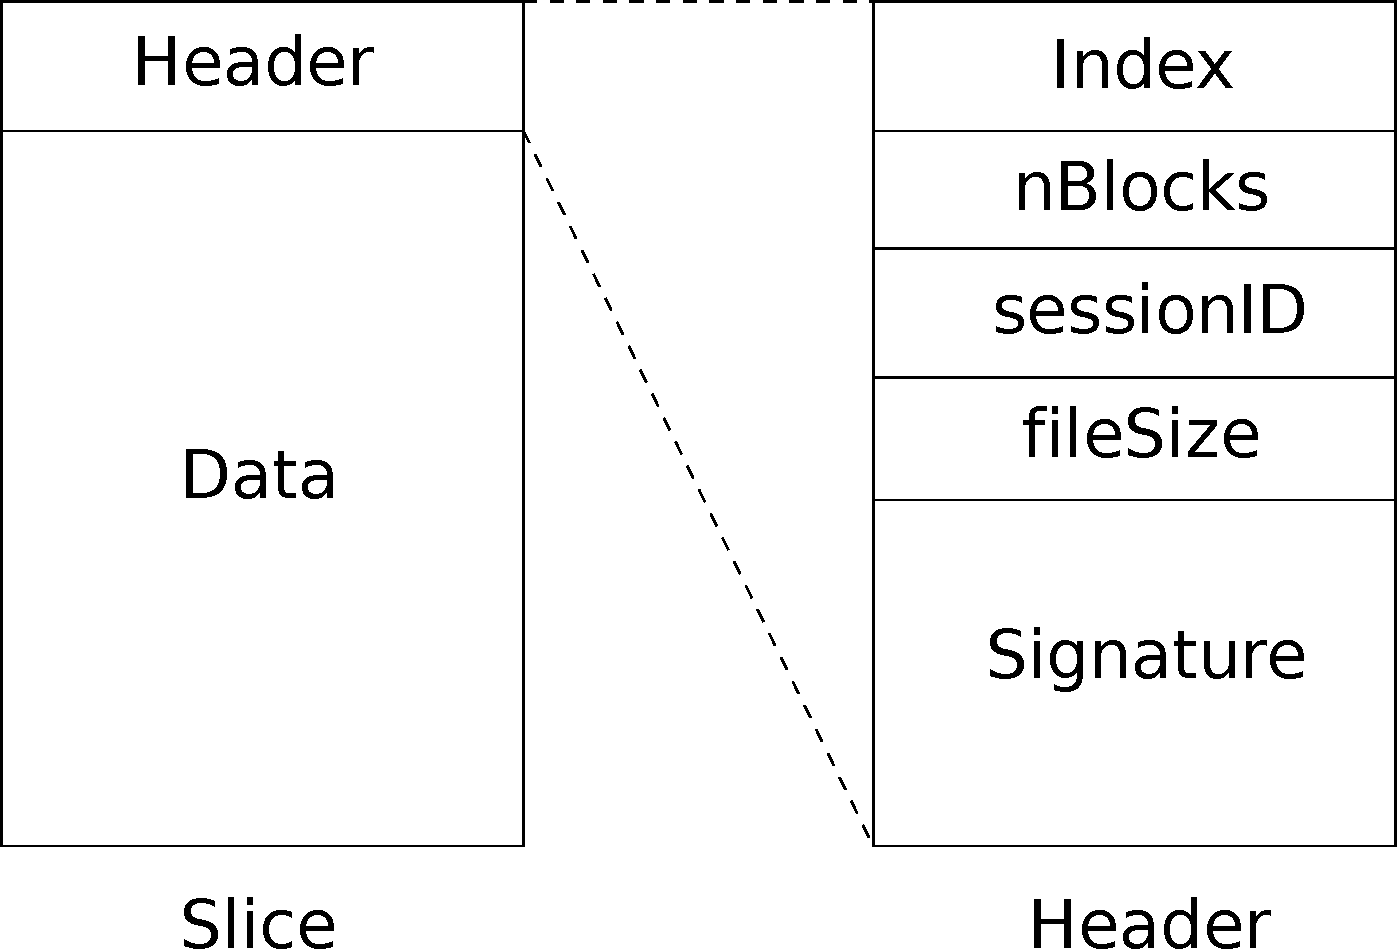
\includegraphics[scale=0.4]{Figures/Slice_Header}
  \decoRule
  \caption[Slice - Header]{Esquema general de las clases Slice y Header}
  \label{fig:Slice_Header}
\end{figure}

\begin{figure}[ht]
  \centering
  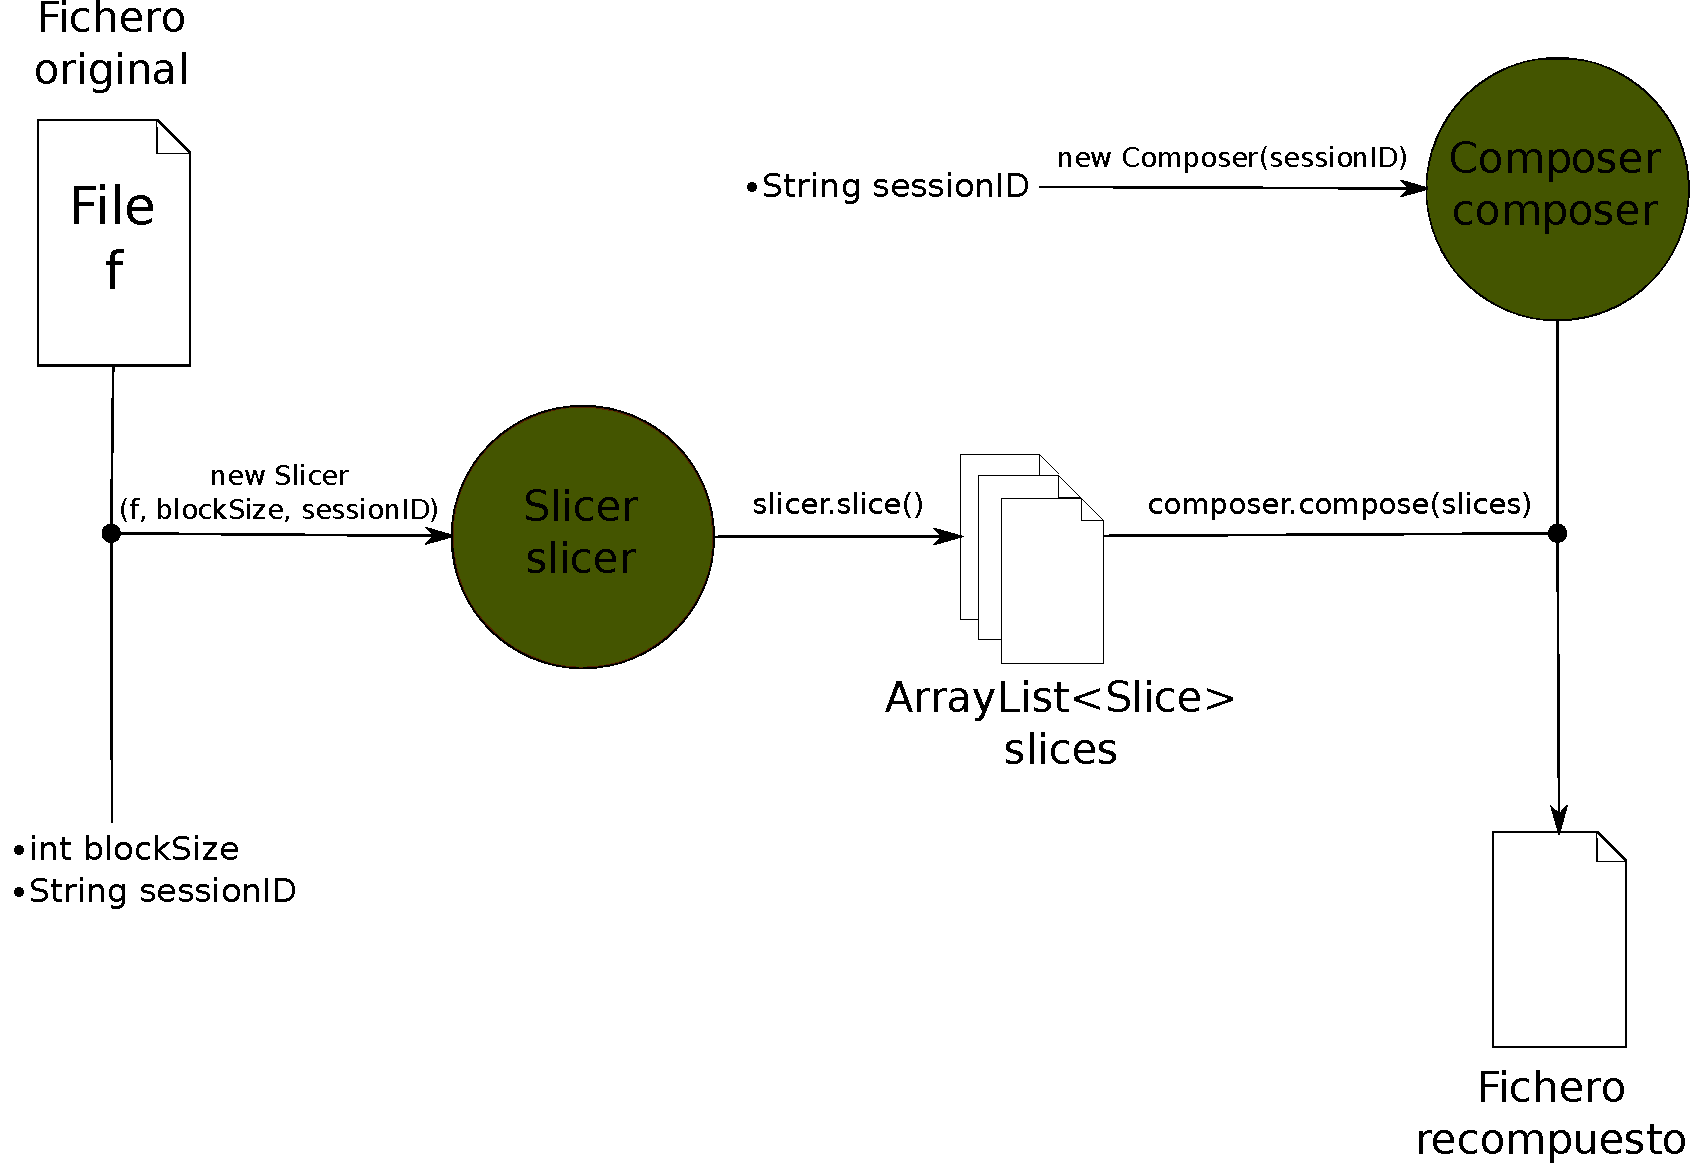
\includegraphics[scale=0.5]{Figures/Assembler}
  \decoRule
  \caption[Slicer - Composer]{Esquema general del Slicer y el Composer}
  \label{fig:Assembler}
\end{figure}

\subsection{Shatter 0.2}

En esta segunda versión, el objetivo era proporcionar confidencialidad a las
Slices. Para llevarlo a cabo se implementaron las siguientes clases:

\begin{itemize}
  \item \keyword{EncFile} -- Viene a ser una Slice cifrada. A parte de los datos
  encriptados de la Slice, también incluye una cabecera (EncFileHeader) con
  algunos datos importantes y una pseudocabecera (FalseHeader) con datos menores.

  \item \keyword{EncFileHeader} -- Como decía antes, esta cabecera se usa para
  almacenar algunos metadatos importantes: el vector de inicialización (IV) que
  se ha usado para cifrar la Slice y una firma para el IV.

  \item \keyword{KeyFile} -- Esta clase se utiliza para almacenar la clave
  simétrica que se ha utilizado para crear los EncFiles. También va firmada.

  \item \keyword{AESLibrary} -- Básicamente, una clase que se encarga de
  generar de manera aleatoria y segura claves simétricas y vectores de
  inicialización.

  \item \keyword{SymmetricCipher} -- Esta es la clase que se encarga de hacer
  la parte más importante en cuanto a la confidencialidad. Una vez que ha sido
  inicializado con una clave simétrica, genera textos cifrados a partir de
  texto plano y un IV. Igualmente, puede llevar a cabo el proceso inverso.

  \item \keyword{Encryptor} -- La \emph{fábrica} de EncFiles. Genera de manera
  aleatoria y segura (Utilizando una de las clases mencionadas anteriormente)
  una clave simétrica para un algoritmo establecido y, con ella, inicializa una
  instancia de un SymmetricCipher. A continuación se le pasa un array de Slices
  del cual genera un array de EncFiles, que es el que retorna.

  \item \keyword{Decryptor} -- La contraparte del Encryptor. Realiza el proceso
  inverso y devuelve un array de Slices a partir de uno de EncFiles.
\end{itemize}

A pesar de que la seguridad que proporciona este prototipo no está completa (Ya
que es propenso a algunos ataques), sienta las bases de lo que es la arquitectura
de seguridad de la aplicación.
